\documentclass[12pt]{extarticle}
\usepackage[utf8]{inputenc}
\usepackage{graphicx}
\usepackage{float}

% Disable indentation
\setlength{\parindent}{0pt}

\title{Lab 5: Configure and Verify a Site-to-Site IPsec VPNUsing CLI}
\author{Alexander Hoffmann}
\date{\today}

\begin{document}

\maketitle

\section{Configure IPsec Parameters on R1}
\subsection{Test connectivity}
\begin{center}
\begin{figure}[H]
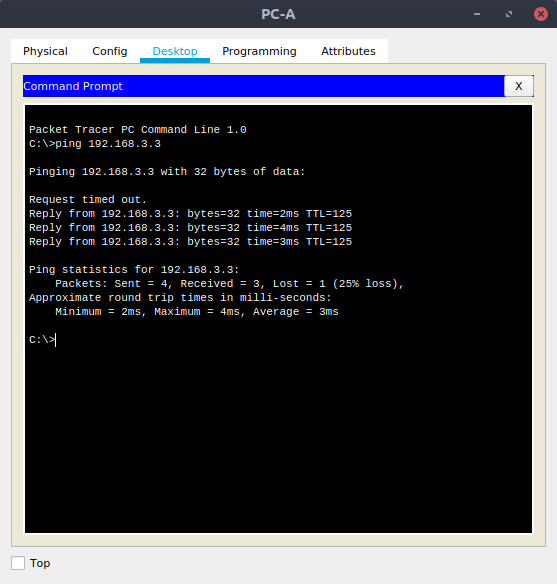
\includegraphics[scale=0.7]{resources/q01a.png}\
\caption{PC-A ping PC-C}
\end{figure}
\end{center}

\subsection{Enable the Security Technology package}
\textbf{a.} On R1, issue the show versioncommand to view the Security Technology package license information.
\begin{center}
\begin{figure}[H]
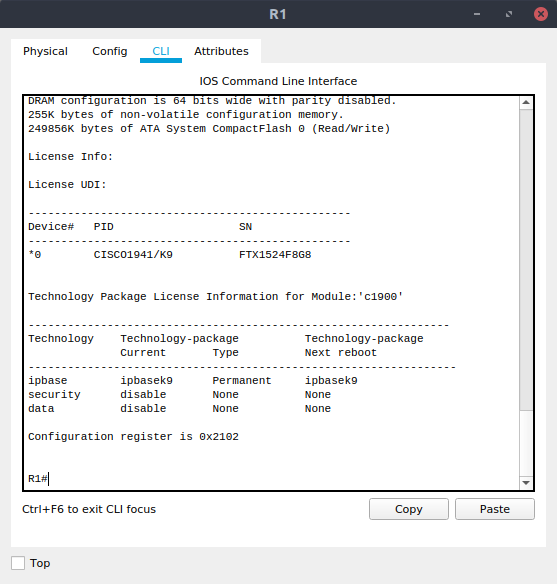
\includegraphics[scale=0.7]{resources/q02a.png}\
\caption{show versioncommand}
\end{figure}
\end{center}

\textbf{b.} If the Security Technology package has not been enabled, use the following command to enable the package.
\begin{center}
\begin{figure}[H]
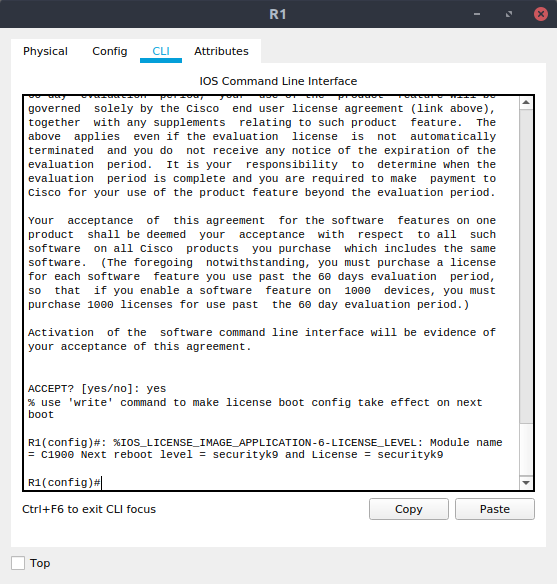
\includegraphics[scale=0.7]{resources/q02b.png}\
\caption{enable Security Technology package}
\end{figure}
\end{center}

\textbf{e.} Verify that the Security Technology package has been enabled by using the show versioncommand.
\begin{center}
\begin{figure}[H]
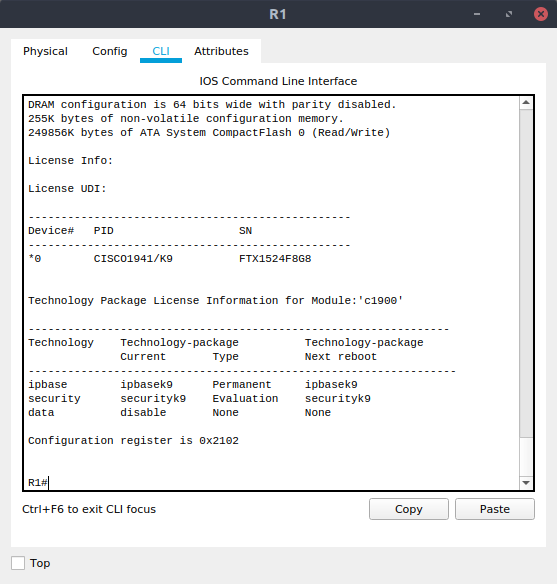
\includegraphics[scale=0.7]{resources/q02e.png}\
\caption{show versioncommand}
\end{figure}
\end{center}

\subsection{Identify interesting traffic on R1}
Configure ACL 110to identify the traffic from the LAN on R1to the LAN on R3as interesting. This interesting traffic will trigger the IPsec VPN to be implemented when there is traffic betweentheR1to R3LANs. All other traffic sourced from the LANs will not be encrypted.Because ofthe implicit deny all, there is no need to configure a deny ip any any statement.

\subsection{Configure the IKE Phase 1 ISAKMP policy on R1}
\begin{verbatim}
R1(config)# crypto isakmp policy 10
R1(config-isakmp)# encryption aes 256
R1(config-isakmp)# authentication pre-share
R1(config-isakmp)# group 5
R1(config-isakmp)# exit
R1(config)# crypto isakmp key vpnpa55 address 10.2.2.2
\end{verbatim}

\subsection{Configure the IKEPhase 2 IPsec policyon R1}
\begin{verbatim}
R1(config)# crypto map VPN-MAP 10 ipsec-isakmp
R1(config-crypto-map)# description VPN connection to R3
R1(config-crypto-map)# set peer 10.2.2.2
R1(config-crypto-map)# set transform-set VPN-SET
R1(config-crypto-map)# match address 110
R1(config-crypto-map)# exit
\end{verbatim}

\subsection{Configure the crypto map on the outgoing interface}
\begin{verbatim}
R1(config)# interface s0/0/0
R1(config-if)# crypto map VPN-MAP
\end{verbatim}

\section{Configure IPsec Parameters on R3}
\subsection{Enable the Security Technology package}
\textbf{b.} Verify that the Security Technology package has been enabled by using the show versioncommand after setting it up.
\begin{center}
\begin{figure}[H]
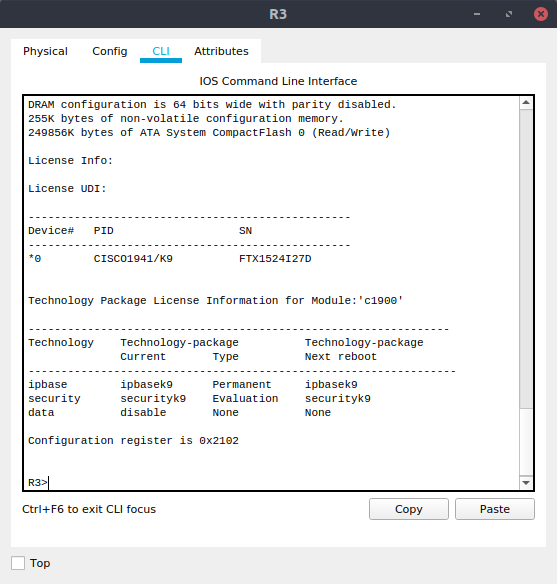
\includegraphics[scale=0.7]{resources/q201b.png}\
\caption{show versioncommand}
\end{figure}
\end{center}

After this, the configuration is similar to the one in the first part. We skip ahead to part 3.

\section{Verify the IPsec VPN}
\subsection{Verify the tunnel prior to interesting traffic}
\begin{center}
\begin{figure}[H]
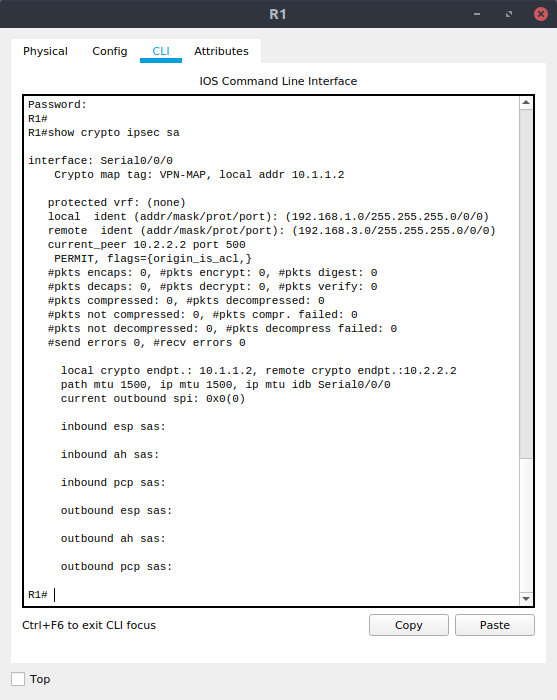
\includegraphics[scale=0.7]{resources/q31.png}\
\caption{show crypto ipsec sa}
\end{figure}
\end{center}

\subsection{Create interesting traffic}
\begin{center}
\begin{figure}[H]
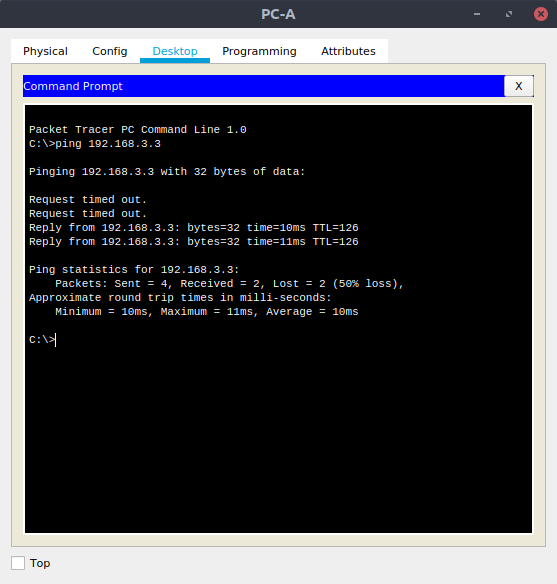
\includegraphics[scale=0.7]{resources/q32.png}\
\caption{Ping PC-C from PC-A}
\end{figure}
\end{center}

\subsection{Verify the tunnel after interesting traffic}
\begin{center}
\begin{figure}[H]
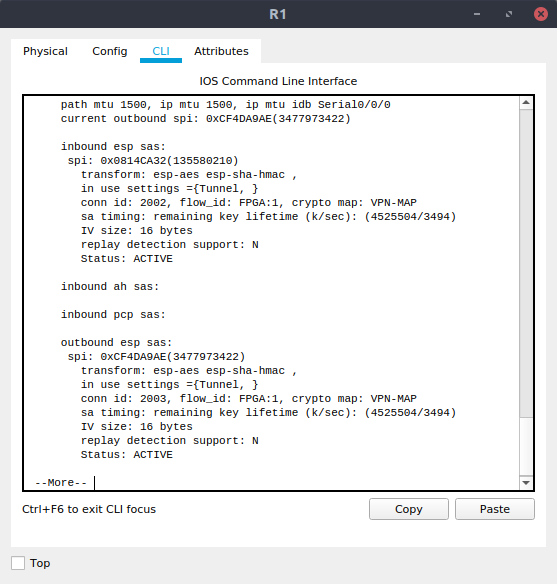
\includegraphics[scale=0.7]{resources/q33.png}\
\caption{show crypto ipsec sa}
\end{figure}
\end{center}

\subsection{Create uninteresting traffic}
\begin{center}
\begin{figure}[H]
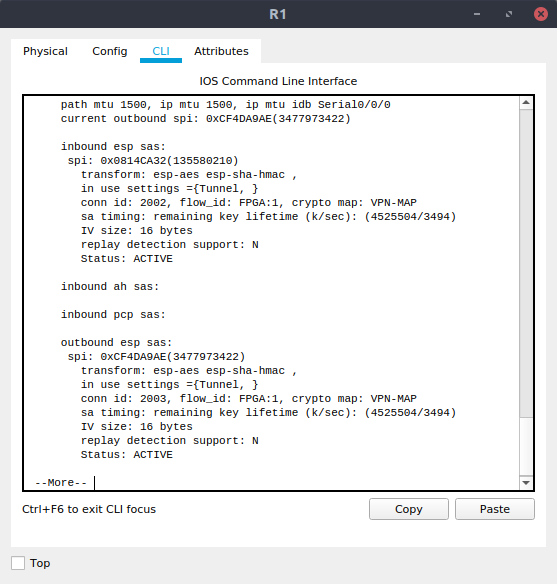
\includegraphics[scale=0.7]{resources/q33.png}\
\caption{show crypto ipsec sa}
\end{figure}
\end{center}

\subsection{Create uninteresting traffic}
\begin{center}
\begin{figure}[H]
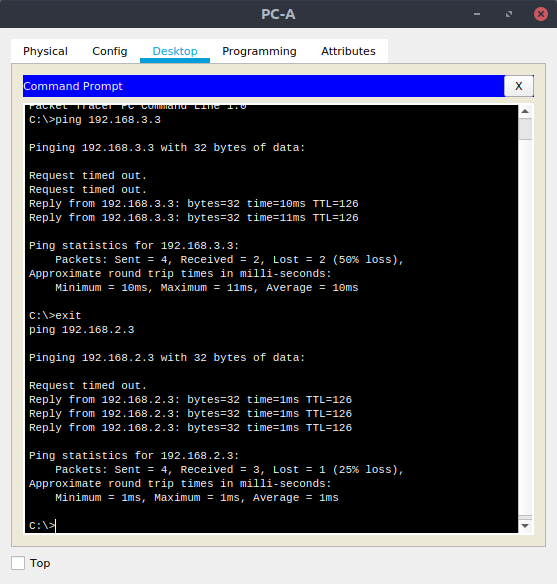
\includegraphics[scale=0.7]{resources/q34.png}\
\caption{Ping PC-B from PC-A}
\end{figure}
\end{center}

\subsection{Verify the tunnel}
\begin{center}
\begin{figure}[H]
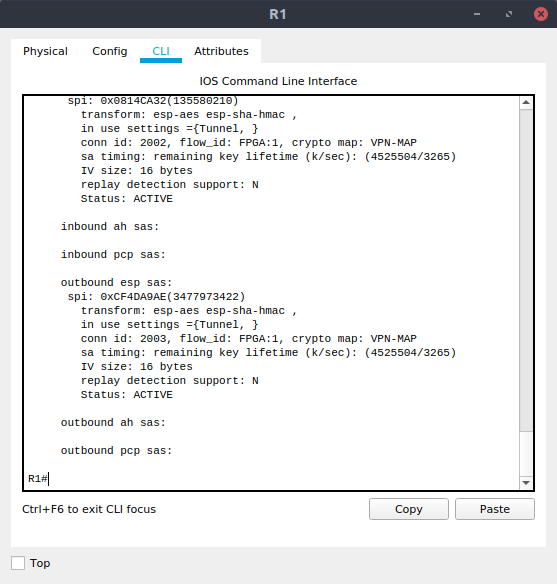
\includegraphics[scale=0.7]{resources/q35.png}\
\caption{show crypto ipsec sa}
\end{figure}
\end{center}

\subsection{Check results}
\begin{center}
\begin{figure}[H]
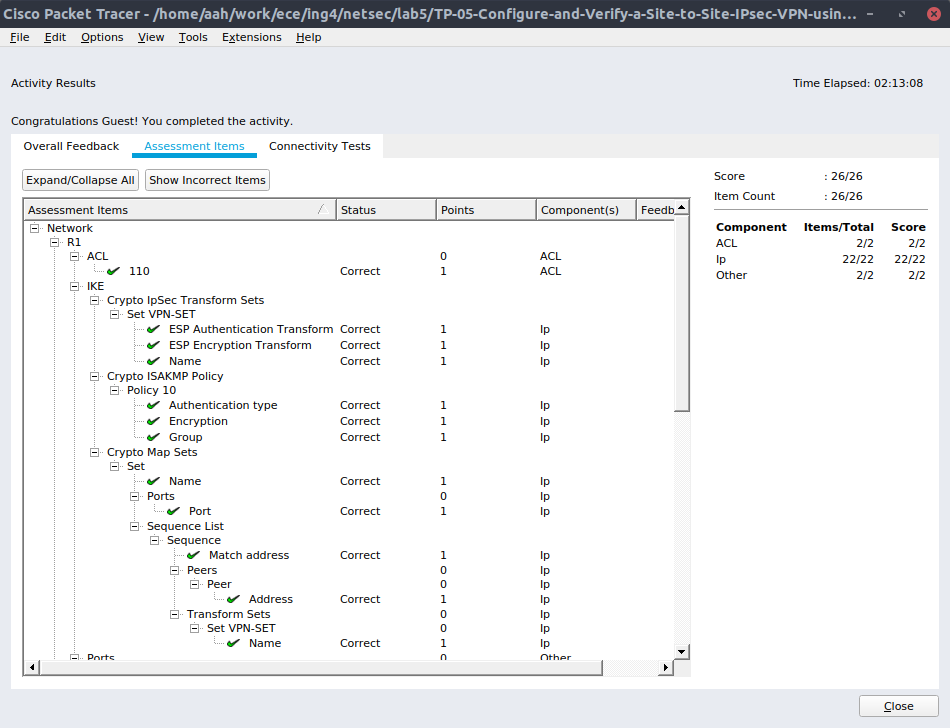
\includegraphics[scale=0.4]{resources/q36.png}\
\caption{Check results}
\end{figure}
\end{center}

\end{document}
